% Created 2016-08-17 Wed 14:38
\documentclass[tikz]{standalone}

\usepackage[utf8]{inputenc}
\usepackage[T1]{fontenc}

\usepackage{circledsteps}

\RequirePackage{xcolor}

%% HPI color definitions according to the design manual
% These do not exactly match the RGB values used in the Powerpoint slide master due to unknown reasons
\definecolor{hpiyellow}{RGB}{246,168,0}
\definecolor{hpiorange}{RGB}{221,97,8}
\definecolor{hpired}{RGB}{177,6,58}
\definecolor{hpigray}{RGB}{90,96,101}
\definecolor{hpiblue}{RGB}{0,122,158}


\renewcommand{\sfdefault}{neosans}
% Different font weights for neosans
\newcommand{\textl}[1]{{\fontseries{l}\selectfont #1}} % light
\newcommand{\textm}[1]{{\fontseries{m}\selectfont #1}} % medium, same as default weight
\newcommand{\textsb}[1]{{\fontseries{sb}\selectfont #1}} % semibold
\newcommand{\textmb}[1]{{\fontseries{mb}\selectfont #1}} % bold, same as \textbf
\newcommand{\texteb}[1]{{\fontseries{eb}\selectfont #1}} % extra bold
\newcommand{\textub}[1]{{\fontseries{ub}\selectfont #1}} % ultra bold

\tikzset{every picture/.style={/utils/exec={\sffamily}}}
\tikzset{flipflop RSflanke/.style={
  flipflop,
  flipflop def={t1=S, t2=C, c2=1, t3=R, t6=Q, t4={\ctikztextnot{Q}}}
}}


\tikzset{
  mechanicalSwitch/.pic={
    \coordinate (-inUp) at (135:2); 
    \coordinate (-inDown) at (235:2);
    \coordinate (-out) at (2,0);
    \coordinate (-center) at (0,0);
    
    \draw (0,0) circle [radius = 2cm];
    \draw [fill=gray!20] (0,0) circle [radius = 0.2cm];

    \draw (0, 0) -- (2, 0);
    \draw (135:.8) -- (135:2); 
    \draw (225:.8) -- (225:2); 

    \draw [fill=gray!20] (2, 0) circle [radius=0.05cm]; 
    \draw [fill=gray!20] (135:2) circle [radius=0.05cm]; 
    \draw [fill=gray!20] (225:2) circle [radius=0.05cm]; 

    
    \draw [thick] (0,0) -- (175:1.5); 

    \draw [dashed, <->, domain=135:225] plot ({cos(\x)}, {sin(\x)}); 
  },
  mechanicalSwitchClosed/.pic={
    \coordinate (-inUp) at (135:2); 
    \coordinate (-inDown) at (255:2);
    \coordinate (-out) at (2,0);
    \coordinate (-center) at (0,0);
    \draw (0,0) circle [radius = 2cm];
    \draw [fill=gray!20] (0,0) circle [radius = 0.2cm];

    \draw (0, 0) -- (2, 0);
    \draw (135:.8) -- (135:2); 
    \draw (225:.8) -- (225:2); 

    \draw [fill=gray!20] (2, 0) circle [radius=0.05cm]; 
    \draw [fill=gray!20] (135:2) circle [radius=0.05cm]; 
    \draw [fill=gray!20] (225:2) circle [radius=0.05cm]; 

    
    \draw [thick] (0,0) -- (135:2); 

    \draw [dashed, <->, domain=135:225] plot ({cos(\x)}, {sin(\x)}); 
  }
}


\usetikzlibrary{calc}
\usetikzlibrary{positioning}


\usetikzlibrary{fit}

\begin{document}

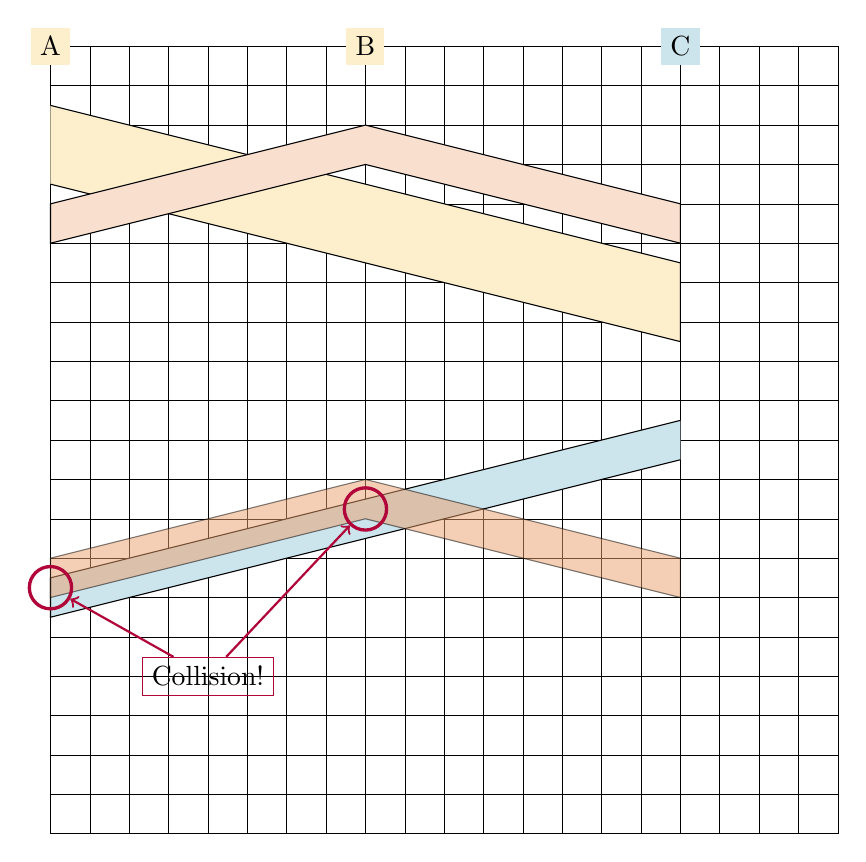
\begin{tikzpicture}

  \draw [step=0.5, very thin] (0,0) grid (10,-10); 
  \node [fill=hpiyellow!20] (a) {A}; 
  \node [fill=hpiyellow!20] (b) at (4,0) {B}; 
  \node [fill=hpiblue!20](c) at (8,0) {C};

  \foreach \n in {a,b,c} \draw (\n) -- ++(0, -10); 

  % packet from A: 
  \draw [fill=hpiyellow!20] (0,-0.75) -- ++(8,-2) -- ++(0,-1) --++ (-8,+2); 

  % packet form B:
  \draw [fill=hpiorange!20] (4,-1) -- ++(4,-1) -- ++(0,-0.5) --++ (-4,+1) -- ++(-4,-1) -- ++(0,0.5) --++(4, 1); 

  % second example
  
  % packet form C:
  \draw [fill=hpiblue!20] (8,-4.75) -- ++(-8,-2) -- ++(0,-0.5) --++ (+8,+2); 

  % packet form B:
  \draw [fill=hpiorange!60, semitransparent] (4,-5.5) -- ++(4,-1) -- ++(0,-0.5) --++ (-4,+1) -- ++(-4,-1) -- ++(0,0.5) --++(4, 1); 

  % collisions:

  \node [draw=hpired, very thick, circle, fit={(0,-6.75)(0,-7)}] (col1) {}; 
  \node [draw=hpired, very thick, circle, fit={(4,-5.75)(4,-6)}] (col2) {}; 
  \node [draw=hpired] at (2,-8) (collabel) {Collision!}; 

  \draw [->, hpired, thick] (collabel) edge (col1) edge (col2); 
  
  
\end{tikzpicture}

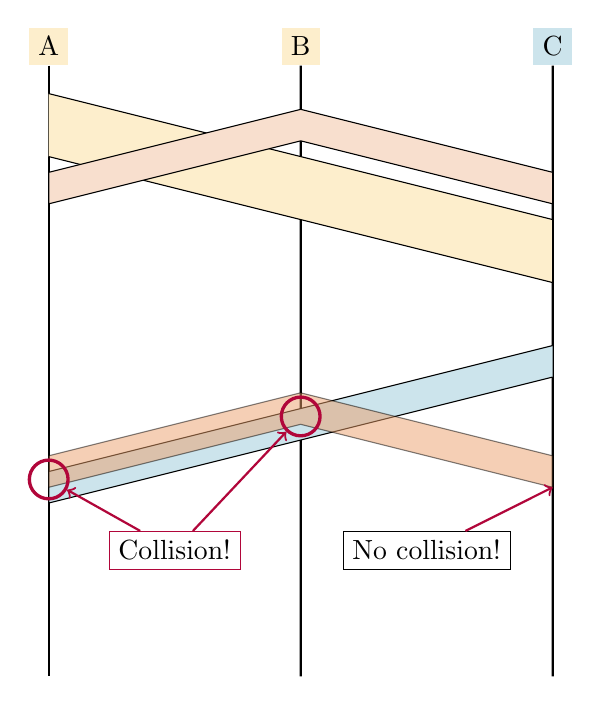
\begin{tikzpicture}[scale=0.8]

%   \draw [step=0.5, very thin] (0,0) grid (10,-10); 
  \node [fill=hpiyellow!20] (a) {A}; 
  \node [fill=hpiyellow!20] (b) at (4,0) {B}; 
  \node [fill=hpiblue!20](c) at (8,0) {C};

  \foreach \n in {a,b,c} \draw [thick] (\n) -- ++(0, -10); 

  % packet from A: 
  \draw [fill=hpiyellow!20] (0,-0.75) -- ++(8,-2) -- ++(0,-1) --++ (-8,+2); 

  % packet form B:
  \draw [fill=hpiorange!20] (4,-1) -- ++(4,-1) -- ++(0,-0.5) --++ (-4,+1) -- ++(-4,-1) -- ++(0,0.5) --++(4, 1); 

  % \onslide<3->

  % second example
  
  % packet form C:
  \draw [fill=hpiblue!20] (8,-4.75) -- ++(-8,-2) -- ++(0,-0.5) --++ (+8,+2); 

  % packet form B:
  \draw [fill=hpiorange!60, semitransparent] (4,-5.5) -- ++(4,-1) -- ++(0,-0.5) --++ (-4,+1) -- ++(-4,-1) -- ++(0,0.5) --++(4, 1); 

  % collisions:

  \node [draw=hpired, very thick, circle, fit={(0,-6.75)(0,-7)}] (col1) {}; 
  \node [draw=hpired, very thick, circle, fit={(4,-5.75)(4,-6)}] (col2) {}; 
  \node [draw=hpired] at (2,-8) (collabel) {Collision!}; 

  \draw [->, hpired, thick] (collabel) edge (col1) edge (col2); 

  
  % no collision  
  % \onslide<4->
  
  \node [draw] at (6,-8) (nocollabel) {No collision!};
  \draw [->, hpired, thick] (nocollabel) -- (8,-7); 

  
\end{tikzpicture}


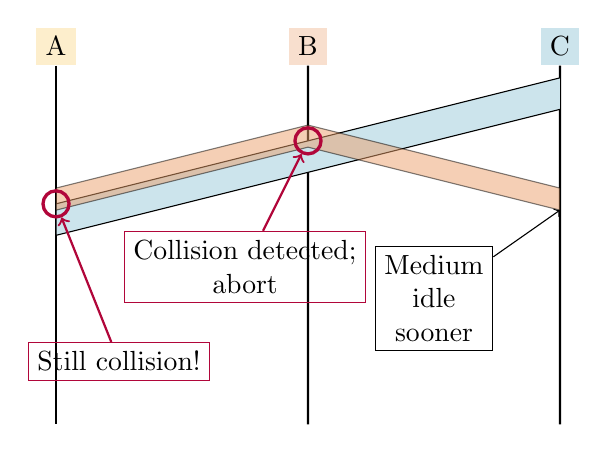
\begin{tikzpicture}[scale=0.8]
  \label{page:mac:collision_detect_msc}
  
  % \draw [step=0.5, very thin] (0,0) grid (10,-10); 
  \node [fill=hpiyellow!20] (a) {A}; 
  \node [fill=hpiorange!20] (b) at (4,0) {B}; 
  \node [fill=hpiblue!20](c) at (8,0) {C};

  \foreach \n in {a,b,c} \draw [thick] (\n) -- ++(0, -6); 

  % second example
  
  % packet form C:
  \draw [fill=hpiblue!20] (8,-0.5) -- ++(-8,-2) -- ++(0,-0.5) --++ (+8,+2); 

  % packet form B:
  \draw [fill=hpiorange!60, semitransparent] (4,-1.25) -- ++(4,-1) -- ++(0,-0.35) --++ (-4,+1) -- ++(-4,-1) -- ++(0,0.35) --++(4, 1); 

  % collisions:

  \node [draw=hpired, very thick, circle, fit={(0,-2.5)(0,-2.5)}] (col1) {}; 
  \node [draw=hpired, very thick, circle, fit={(4,-1.5)(4,-1.5)}] (col2) {}; 

  \node [draw=hpired, align=center] at (3,-3.5) (collabelleft) {Collision detected;\\ abort}; 

  \node [draw=hpired] at (1,-5) (collabelright) {Still collision!}; 

  \draw [->, hpired, thick] (collabelleft) edge (col2);
  \draw [->, hpired, thick] (collabelright) edge (col1); 

  \node [align=center, draw] at (6,-4) (medium_idle) {Medium\\ idle\\ sooner};
  \draw [<-] (8,-2.6) -- (medium_idle); 
  
  

  
\end{tikzpicture}


\end{document}